\documentclass[a4paper, 12pt]{report}


\usepackage[spanish]{babel}
\usepackage[utf8]{inputenc}
\usepackage{textcomp}
\usepackage{booktabs}
\usepackage{amssymb}
\usepackage{bussproofs}
\usepackage{fancyhdr}
\usepackage{graphicx}
\usepackage{amsmath}

\usepackage{hyperref}
\hypersetup{
    colorlinks=true,
    linkcolor=blue,
    filecolor=magenta,
    urlcolor=cyan,
}

\pagestyle{fancy}
\lhead{Almeida, Figueroa \& Ibarra}
\chead{Tarea 1}
\rhead{\today}

\begin{document}
\begin{titlepage}
    \centering
    {\scshape\Huge Universidad Nacional Autónoma de México \par}
    \vspace{1.25cm}
    {\scshape\huge Fundamentos de Bases de Datos\par}
    \vspace{1.25cm}
    {\huge\bfseries Tarea 1: Conceptos Básicos\par}
    \vspace{1.25cm}
    {\Large\textsc Almeida Rodríguez Jerónimo\par}
    \vspace{.1cm}
    {\large\texttt{418003815}\par}
    \vspace{0.25cm}
    {\Large\textsc Figueroa Sandoval Gerardo Emiliano\par}
    \vspace{.1cm}
    {\large\texttt{315241774}\par}
    \vspace{0.25cm}
    {\Large\textsc Ibarra Moreno Gisselle \par}
    \vspace{.1cm}
    {\large\texttt{315602193}\par}
    \vspace{1.5cm}
    \vfill
    \begin{figure}[hb!]
        
\includegraphics[width=.3\textwidth]
            {../logos/escudo_f-ciencias.png}\hfill
        
\includegraphics[width=.3\textwidth]
            {../logos/Escudo_UNAM.png}\hfill
    \end{figure}
\end{titlepage}
\begin{enumerate}
\item[1)]{
\begin{enumerate}
    \item[a)]{¿Por qué elegirías almacenar datos en un sistema de base
	 de datos en lugar de simplemente almacenarlos utilizando el
	 sistema de archivos de un sistema operativo? ¿En qué casos no
	 tendría sentido utilizar un sistema de base de datos?\\

	 No podría guardar cantidades grandes de información, el acceso
	 y las busquedas de información grandes	toman demasiado tiempo
	 en un sistema de archivos.Tampoco se pueden ordenar y actualizar
	 constantemente, tampoco podría modificar el esquema de la base
	 de datos sin tener que modificar completamente los archivos.\\
	 El sistema de archivos no es seguro incluso con un sistema
	 de contraseñas ya que no podemos asegurar la integridad de los
	 datos. No es dinámico, para que más personas tuvieran acceso a
	 mi base de datos tendría que pasarles los datos manualmente, lo cual es muy ineficiente.\\
	 No tendría sentido usar una base de datos cuando se tienen muy
	 pocos datos a guardar.}
    \item[b)]{¿Qué ventajas y desventajas encuentras al trabajar con una
	 base de datos?\\
	 \textbf{Ventajas:}
	 \begin{itemize}
	 	\item Se pueden sincronizar datos en ella
	 	\item Se puede modificar la estructura fácilmente
	 	\item Garantizan la fiabilidad
	 	\item Existen por un periodo largo de tiempo
	 	\item Permite controlar la redundancia
	 	\item Son independientes a los programas que proporcionan las
	 	vistas.
	 \end{itemize}
 	 \textbf{Desventajas:}
 	 \begin{itemize}
 	 	\item Son costosas.
 	 	\item No cualquiera puede manejarla, se necesita alguien
 	 	especializado.
 	 	\item Se requiere de capacitación para su manejo.
 	 \end{itemize} }

    \item[c)] Investiga cuáles serían las responsabilidades de un DBA y las de un diseñador de bases de datos.\\
    \textbf{Responsabilidades de un DBA:}
    \begin{itemize}
    	\item Hacer copias de seguridad y la recuperación de estas:\\
    	El administrador debe hacer copias de seguridad periódicas y tener conocimiento completo del procedimiento de restauracíon.
    	\item La Supervisión de la actividad de las bases de datos:\\
    	El administrador debe de saber cuándo se producen retrotracciones de transacciones, cuándo  la base de datos supera el espacio en disco del sistema, cuándo no se respetan restricciones exclusivas o cuándo no se debe cerrar la base de datos mientras la aplicación se está ejecutando por mencionar algunas.
    	\item Checar el Rendimiento:\\
    	El administrador debe actuar de inmediato cuando se ven problemas con el rendimiento , supervisar cuándo realiza la base de datos una retrotracción en una transacción de gran tamaño (ya que causa otros problemas de rendimiento en otras areas), comprobar si la base de datos se está ejecutando de manera optimizada, no sólo en el nivel del sistema sino también en el nivel de las tablas y las consultas, calcular con qué frecuencia se tienen que actualizar las estadísticas para obtener un rendimiento óptimo o reorganizar las tablas y los índices a intervalos de tiempo regulares.
    	\item Checar por Bloqueos:\\
    	El administrador debe analizar de dónde provienen dichos bloqueos, detecta puntos muertos o sino comprueba por qué el origen del bloqueo sigue bloqueando.
    \end{itemize}
    \textbf{Responsabilidades de un Diseñador de Base de Datos:}
    \begin{itemize}
    	\item Diseño de base de datos:\\
    	El diseñador debe Garantizar que los datos persistentes se almacenan de forma coherente y eficaz ademas de definir el comportamiento que se debe implementar en la base de datos.
    	\item Identificar ideas de prueba:\\
    	El diseñador debe indentificar las ideas de prueba que se deben explorar para valorar la calidad aceptable de los elementos de prueba de destino como tambien identificar un número suficiente de ideas para validar de forma adecuada elementos de prueba de destino con motivadores de prueba.
    	\item Implementar elementos de diseño:\\
    	El diseñador debe producir una implementación para una parte del diseño (por ejemplo, una clase, una realización de guión de uso o una entidad de base de datos), o para solucionar uno o varios defectos.
    	\item  Revisar el diseño:\\
    	El diseñador debe verificar que el modelo de diseño cumple los requisitos del sistema y que es una buena base para su implementación, garantizar que el modelo de diseño es coherente con las directrices de diseño generales y que las directrices de diseño cumplen sus objetivos.


    \end{itemize}

    \item[d)] Investia  cuáles  serían  los distintos tipos de
     usuarios finales de una base de datos, indica las principales
     actividades que realizaría cada uno de ellos. \\\\
     \textbf{Usuarios Finales.} Acceden a la base de datos desde
     alguna terminal, pueden utilizar un lenguaje de consultar o un
     programa de aplicación. Tenemos distintos tipos de usuarios
     finales:
     \begin{itemize}
       \item \textbf{Esporádicos.} Acceden de vez en cuando, no
       siempre requieren la misma información. Utilizan lenguajes
       sofisticados de consulta para especificar su solicitud.\\
       \item \textbf{Paramétricos.} Estos usuarios hacen consultas
       y actualizan la base de datos constantemente, no necesitan
       aprender del lenguaje de consultas, ya que normalmente
       utilizan una interfaz gráfica diseñada para ese propósito.
       \item \textbf{Sofisticados o avanzados.} Son profesionales,
       tales como ingenieros, científicos y otros que están muy
       familiarizados con el sistemas manejador de bases de datos.
       Estos usuarios suelen hacer uso de sus conocimientos para
       satisfacer requerimientos complejos.
       \item \textbf{Autónomos.} Mantienen sus propias bases de datos, utilizando paquetes de programas que facilitan su uso.

     \end{itemize}
    \item[e)]{Explica las diferencias entre la independencia de datos física y
                lógica. ¿Cuál es más difícil de lograr y por qué?\\
        La indpenedencia de datos lógica se refiere al modelo del esquema bajo el
        cual se van a organizar los datos en la base de datos. Por otro lado,
        la independecia física es la manera en la que los datos en sí son almacenados
        en el dispositivo de almacenamiento, ya sea un disco duro o similar.
        La independencia de estos dos niveles se refiere a que al momento de
        actualizar la información alterando un nivel, el otro no se vea afectado.\\
        La independencia lógica es más difícil de lograr porque hay que modelar los
        esquemas de tal manera que la información sea clara, concisa, entendible y no
        redundante. También al modificar el esquema lógico hay que tomar en cuenta cómo
        se van a obtener los datos que no se tenían antes de esta modificación.
    }
    \item[f)]{¿Qué es el diccionario de datos y por qué es importante para el SMBD?}\\
    Un diccionario de datos es un conjunto de metadatos que contiene las características lógicas de los datos que se van a utilizar en el sistema que se programa, incluyendo nombre, descripción, alias, contenido y organización.Estos diccionarios se desarrollan durante el análisis de flujo de datos y ayuda a los analistas que participan en la determinación de los requerimientos del sistema, su contenido también se emplea durante el diseño del proyecto.Identifica los procesos donde se emplean los datos y los sitios donde se necesita el acceso inmediato a la información, se desarrolla durante el análisis de flujo de datos y auxilia a los analistas que participan en la determinación de los requerimientos del sistema, su contenido también se emplea durante el diseño.El objetivo de un diccionario de datos es dar precisión sobre los datos que se manejan en un sistema, evitando así malas interpretaciones o ambigüedades.
    \item[g)]{Indica las principales características de los modelos de
    datos más representativos. ¿Cuáles serían las diferencias
    entre los  modelos relacional, orientado a objetos,
    semiestructurado y objeto –relacional?\\
    \textbf{Modelo Relacional.}Los datos se perciben como tablas,
    es un sistema cerrado, todas las operaciones son siempre tablas.\\
    \textbf{Modelo Orientado a Objetos.} Los datos se modelan como
    objetos, se tiene comportamiento (métodos o funciones) y estado.\\
    \textbf{Modelo Semiestructurado.} Es una colección de nodos y
    cada nodo tiene datos con diferentes esquemas, esto lo hace un
    sistema menos rígido.\\
    \textbf{Modelo Objeto-Relacional} Representa los datos como tablas,
    permite construir tipos de objetos complejos, capacidad para
    encapsular y asociar métodos a los objetos.}
    \item[h)]{Elabora una línea de tiempo, en dónde indiques los principales
              hitos en el desarrollo de las BDs.\\
        \begin{figure}[ht!]
            \centering
            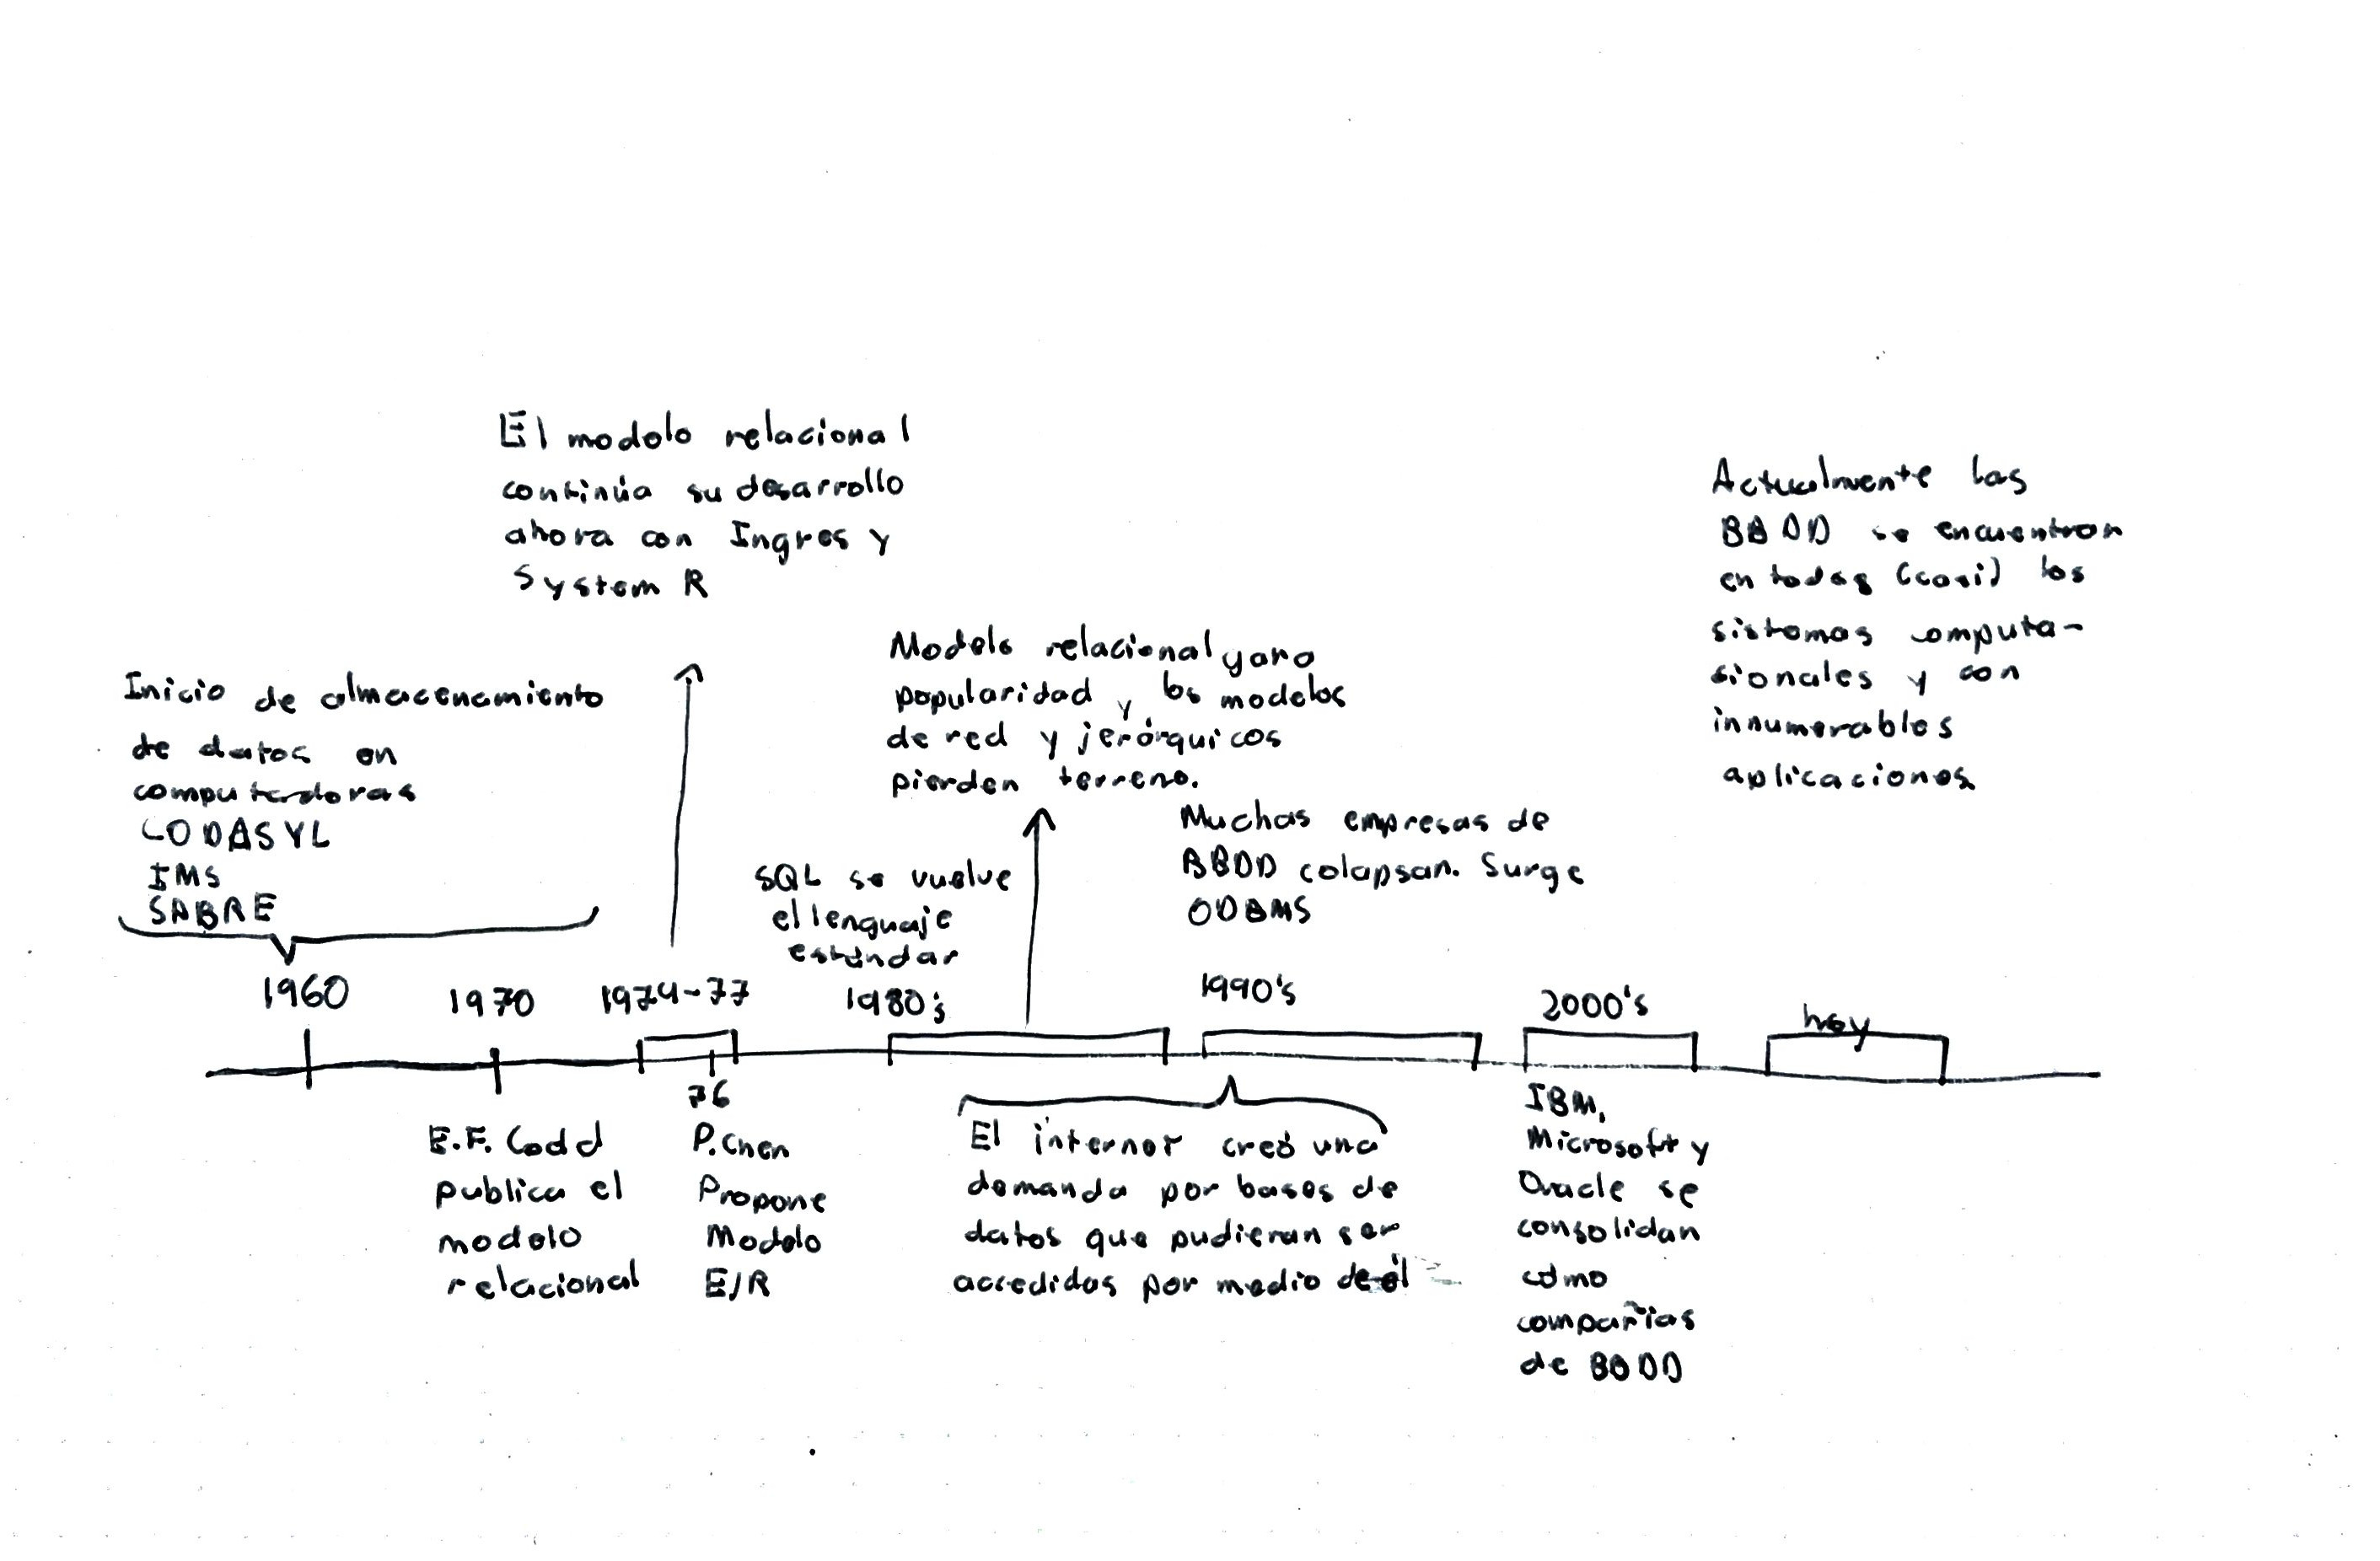
\includegraphics[width=\textwidth]{Linea_de_tiempo_BD.jpg}
            \caption{Línea de tiempo }
        \end{figure}
        Línea de tiempo basada en la información obtenida de: \cite{DBH}
    }
    \item[i)]{Indica las responsabilidades que tiene un Sistema Manejador de
                Bases de Datos y para cada responsabilidad, explica los problemas
                que surgirían si dicha responsabilidad no se cumpliera.\\
        Responsabilidades:\\
        \begin{enumerate}
            \item{Interacción con el administrador de archivos}
            \item{Cuidar de la integridad y seguridad de los datos}
            \item{Respaldo y recuperación}
            \item{Control de concurrencia}
        \end{enumerate}
        Sin poder interactuar con el sistema administrador de archivos es imposible
        guardar y recuperar los datos.\\
        En caso de que el SMBD no cuide de la integridad y seguridad de los datos
        pueden surgir problemas del tipo que alguna persona no deseada pueda acceder
        y mulipular los datos (seguridad) o de que los datos se hayan corrompido
        (integridad).\\
        Sin respaldo y recuperación surge el problema de que se puedan perder los
        datos de manera permanente.
        Finalmente, sin un control de concurrencia correcto, surge el problema de
        que se intente acceder a la información desde diversos puntos ya sea para
        leerla o modificarla pero con el problema de que ambas lecturas puedan
        ser distintas.
        \cite{RDBMS}
    }
    \item[j)]{Supón  que  un banco pequeño desea  almacenar  su
    información  en una  base  de  datos  y  le gustaría comprar
    el SMBD que  tenga  la  menor  cantidad  de  características
    posibles. Está interesado en ejecutar la aplicación en una sola computadora personal y no se planea compartir la
    información  con  nadie.  Para  cada  una  de  las
    siguientes  características  explica  por  qué  se debería o
    no incluir en el SMBD que se desea comprar (suponiendo que se
    pueden comprar por separado): \textbf{seguridad, control de
    concurrencia, recuperación en caso de fallas, lenguaje de
    consulta, mecanismo de vistas, manejo de transacciones}\\
    \textbf{Seguridad:} Es necesario comprarlo, ya que no quieren
    compartir la información con nadie, por lo tanto los datos
    se deben proteger y evitar que cualquiera pueda acceder a
    ellos.\\
    \textbf{Control de concurrencia:} No se necesita incluir ya que
    se planea ejecutar la aplicación en una sola computadora
    personal, por lo que el control de concurrencia sería
    completamente innecesario si no va a ser utilizados por varias
    personas a la vez.\\
    \textbf{Recuperación en caso de fallas:} Es necesario, ya que
    la aplicación solo funcionará en una sola computadora personal,
    por lo que si hubiera algún tipo de falla, toda la información
    se perdería y no habría ningún otro lugar para recuperarlo.\\
    \textbf{Lenguaje de consulta:} Es necesario, para poder acceder,
    actualizar y guardar los datos en la base de datos.\\
    \textbf{Mecanismo de vista}\\
    \textbf{Manejo de transacciones}No es necesario\\}
\end{enumerate}
}
\item[2)]{
\begin{enumerate}
    \item[a)]{¿Qué es la Calidad de Datos y cómo se relaciona con las
    bases de datos?\\
    Es  el estado de completez, validez, consistencia y exactitud
    que hace a los datos apropiados para su uso. También puede ser
    definida como el grado en el que un conjunto de características
    cumplen con los requerimientos necesarios.
    Se relaciona con las bases de datos ya que una buena calidad de
    datos es esencial en la resolución de entidades, ya que aumenta la
    fiabilidad de las entidades resueltas y las relaciones
    detectadas.Muchos problemas que se suelen presentar en una base
    de datos se pueden solucionar con una buena calidad y manejo
    de datos. Además esto reduce costos a la larga.
}
    \item[b)]{¿Qué son las bases de datos NoSQL? indica el modelo de datos utilizado y algunos proveedores. }\\

    Son una amplia clase de sistemas de gestión de bases de datos que difieren del modelo clásico de SGBDR (Sistema de Gestión de Bases de Datos Relacionales) en aspectos importantes, siendo el más destacado que no usan SQL como lenguaje principal de consultas. Los datos almacenados no requieren estructuras fijas como tablas, normalmente no soportan operaciones JOIN, ni garantizan completamente ACID (atomicidad, consistencia, aislamiento y durabilidad). No tienen un modelo predeterminado como era el relacional en los SGBDR, sino se adapta segun la cantidad y tipo de datos que se vayan a utilizar para asi llegar a algo mucho mas optimizado , mientras mas aumente la estructura y más escalable se quiere hacer un proyecto, más cuesta conseguir que una base de datos relacional sea intuitiva, por no hablar de la dificultad para conservar su simplicidad.\\
    Algunos proveeedores serian :
    \begin{itemize}
    	\item MongoDB
    	\item Cassandra
    	\item Amazon DynamoDB
    	\item Oracle NoSQL
    	\item Redis
    	\item etc...
    \end{itemize}
    \item[c)]{Un almacén de datos es cómo una base de datos superpoderosa. Su
        propósito es almacenar grandes cantidades de datos, entre ellos de tipo
        histórico, con el fin de hacer análisis sobre cantidades de información
        grandes y distintas. La diferencia con una base de datos es que la base
        de datos se enfoca en almacenar y recuperar información específica del
        contexto en el que se desempeña. Por su parte, el almacén de datos almacena
        información mucho más diversa y su uso es más amplio.\cite{DWvDB}
    }



\end{enumerate}
}
\end{enumerate}
\begin{thebibliography}{20}
    \bibitem[DBA]{DBA}
        Wikipedia. (2019).\\
        Administrador de Banco de Dados.\\
        Visitado el 22 de agosto del 2019.\\
        \url{https://pt.wikipedia.org/wiki/Administrador_de_banco_de_dados}
    \bibitem[DBD]{DBD}
        Wikipedia. (2019).\\
        Database design.\\
        Visitado el 23 de agosto del 2019.\\
        \url{https://en.wikipedia.org/wiki/Database_design}
    \bibitem[DI]{DI}
        tutorialspoint. (2019).\\
        DBMS - Data Independence.\\
        Visitado el 23 de agosto del 2019.\\
        \url{https://www.tutorialspoint.com/dbms/dbms_data_independence.htm#}
    \bibitem[DI2]{DI2}
        Wikipedia. (2019).\\
        Data independence.\\
        Visitado el 23 de agosto del 2019.\\
        \url{https://en.wikipedia.org/wiki/Data_independence}
    \bibitem[RDBMS]{RDBMS}
        GTU MCA Course Site. (2019).\\
        Responsibilities of Database Management System.\\
        Visitado el 23 de agosto del 2019.\\
        \url{https://sites.google.com/site/gtublog/sem2/2620003/responsibilitiesofdbms}
    \bibitem[DW]{DW}
        Wikipedia. (2019).\\
        Data warehouse.\\
        Visitado el 23 de agosto del 2019.\\
        \url{https://en.wikipedia.org/wiki/Data_warehouse}
    \bibitem[DWvDB]{DWvDB}
        panoply. (2019).\\
        The Difference Between a Data Warehouse and a Database.\\
        Visitado el 23 de agosto del 2019.\\
        \url{https://panoply.io/data-warehouse-guide/the-difference-between-a-database-and-a-data-warehouse/}

    \bibitem[DBH]{DBH}
        quickbase. (2019).\\
        A Timeline of Database History.\\
        Visitado el 23 de agosto del 2019.\\
        \url{https://www.quickbase.com/articles/timeline-of-database-history}

\end{thebibliography}
\end{document}
